%!TEX root = practicum1.tex
Artificial neural networks are non-linear mapping systems inspired by biological nervous systems. The most import parts of a biological neuron include a dendrite that receives signals from other neurons, and a soma that integrates the signals and generates a response that is distributed via a branching axon. 

An artificial neural network consists of a large numbers of simple processors linked by weighted connections, analogously the neurons. Each processor receives inputs from many other nodes and generates a single scalar output that depends on locally available information. This scalar is distributed as input to other nodes. \\

The most simple case of a neural network is the single-layer perceptron, see \autoref{fig:1:perceptron}. This network consists of one layer of input nodes connected to a processing unit through a single layer of weights, which determine the result of the output node. Mathematically a single-layer perceptron is a feed-forward network of nodes with a response function $f(\vec{w}^T\vec{x})$ where $\vec{w}$ is the vector of weights, $\vec{x}$ is the pattern and $f$ is a sigmoid squashing function\cite{reed1998neural}. This squashing function ensures the binary output of the perceptron. \\

The perceptron is a linear binary classifier, which means that is separates classes with a hyperplane, as a consequence perceptrons can only separate linearly separable datasets. We identify two different types of linearly separable datasets: homogeneously separable data sets can be separated by a hyperplane through the origin, inhomogeneously separable data sets cannot be separated by a hyperplane through the origin but they can be separated by a hyperplane if it is offset with a certain bias with respect to the origin. This bias can be incorporated into the network by adding a fixed input of minus one and the bias as the weight connected to this fixed input. Thus we will make no distinction between homogeneously and inhomogeneously separable datasets and talk about linearly separable sets \cite[Chapter 4]{rojas1996neural}.

\begin{figure}[H]
	\centering
	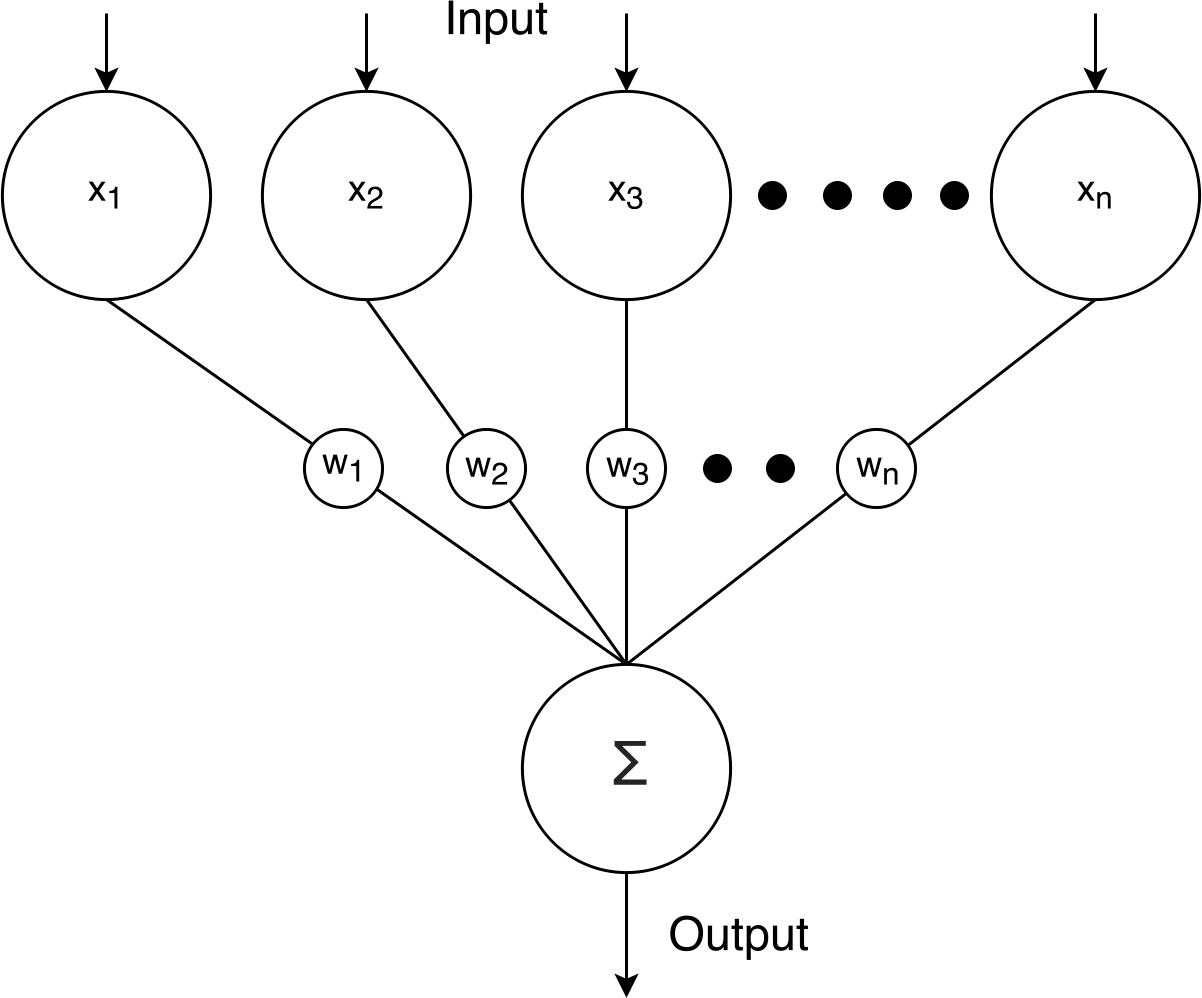
\includegraphics[width=\columnwidth]{./img/perceptron}
	\caption{A perceptron.}
	\label{fig:1:perceptron}
\end{figure}

It can be shown that the perceptron converges, i.e. it separates positive examples for the negatives, if the input data set is linearly separable. \todo[inline]{Reference to book with the proof}

In this paper we will consider the Rosenblatt algorithm for perceptron training. \todo[inline]{Referentie naar het experiment}



